%-*-coding:utf-8-*-
%%%%%%%%%%%%%%%%%%%%%%%%%%%%%%%%%%%%%%%%%%%%%%%%%%%%%%%%%%%%%%%%%%%%%%%%%%%%%%%%
%% Name:   Work Report                                                        %%
%% Author: Wolfson                                                            %%
%% Date:   2021-10-13                                                         %%
%% Discription:                                                               %%
%%%%%%%%%%%%%%%%%%%%%%%%%%%%%%%%%%%%%%%%%%%%%%%%%%%%%%%%%%%%%%%%%%%%%%%%%%%%%%%%


\begin{frame}
  \maketitle
\end{frame}

\section*{Contents}

\begin{frame}{Contents}
  \tableofcontents
\end{frame}

\section{Itermize}

\begin{frame}{Contents}
  \tableofcontents[currentsection]
\end{frame}

\begin{frame}{Test}
  \begin{itemize}
  \item one thing
  \item another thing
  \end{itemize}
\end{frame}

\section{Figure}

\begin{frame}{Contents}
  \tableofcontents[currentsection]
\end{frame}

\begin{frame}{Test}
  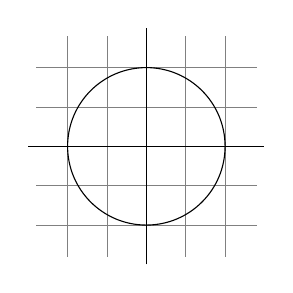
\begin{tikzpicture}
    \draw[step=.5cm,gray,very thin] (-1.4,-1.4) grid (1.4,1.4);
    \draw (-1.5,0) -- (1.5,0);
    \draw (0,-1.5) -- (0,1.5);
    \draw (0,0) circle [radius=1cm];
  \end{tikzpicture}
\end{frame}


%% -----------------------------------------------------------------------------
\appendix


%%%%%%%%%%%%%%%%%%%%%%%%%%%%%%%%%%%%%%%%%%%%%%%%%%%%%%%%%%%%%%%%%%%%%%%%%%%%%%%%
\endinput
